\documentclass{article}
%\documentclass{IEEETran}

%\usepackage{anysize}
%\usepackage[left=1.9cm,right=1.9cm,top=2.54cm,bottom=1.9cm]{geometry}
%\usepackage{sectsty}
%\sectionfont{\normalsize \bf}
%\subsectionfont{\normalsize \bf}

%\IEEEoverridecommandlockouts  
%\overrideIEEEmargins

%\usepackage{siunitx}
\usepackage{setspace} 
%\doublespacing
\usepackage{cite}
\usepackage{amsmath}
\usepackage{amsthm}
\theoremstyle{remark}
\newtheorem{assumption}{Assumption}
\theoremstyle{remark}
\newtheorem{remark}{Remark}
\theoremstyle{remark}
\newtheorem{theorem}{Theorem}
\theoremstyle{remark}
\newtheorem{lemma}{Lemma}
\theoremstyle{remark}
\newtheorem{property}{Property}
\theoremstyle{remark}
\newtheorem{definition}{Definition}
\usepackage{graphicx}
\usepackage{fancyhdr}
\usepackage[bottom]{footmisc}
\usepackage{hyperref}
\usepackage{amssymb}
\usepackage{enumerate}
%===================================

\title{ Optimal Control of An Invasive Plant in n-D Action Space}


\author{Soheil}
\begin{document}
\maketitle
\section{Problem Definition}
In this research we study the optimal control of \textbf{Glossy Buckthorn}, an invasive plant in the area of New England. The mathematical equation that governs the problem is driven based upon the plant's growing cycle, from when they are seeds to when their fruits are being eaten by other animals, such as birds and rats, and their seeds, again, are being spread to miles away by these animals. In figure \ref{fig:outline}, the whole process is outlined by details.For more elaborate explanation please refer to \href{https://github.com/rlsquared/gbPopMod}{here}.

\begin{figure}
\centering
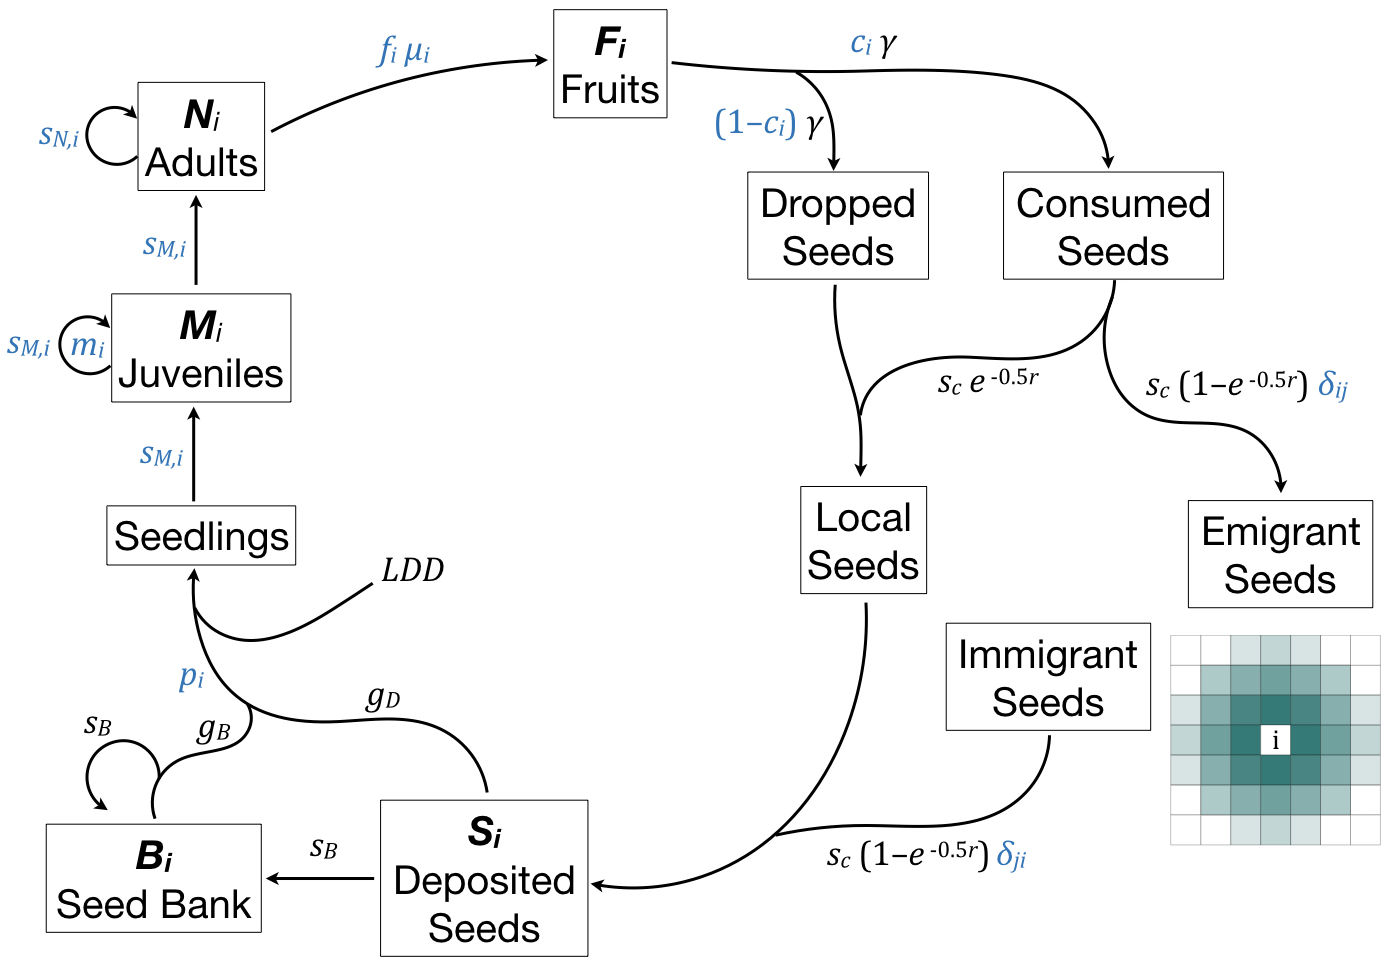
\includegraphics[scale=.2]{model_outline.jpeg}
\label{fig:outline}
\caption{The cycle outline}
\end{figure}

We are trying to solve this problem as a Markov Decision Process. Since, in the first step, we are finding the most basic solution to the problem, we consider the states, actions, rewards, and transition probabilities in its most simplified shape, as follows;

\begin{itemize}
 \item States: The number of the plant in the whole region, the number of week in a year, the number of other important plans that we might be interested to consider (or possible be affected by the efforts of controlling our plant).
 \item Actions: Not taking action, spraying pesticide, cutting the plant, growing native competitor plants, spreading mulch, burning the plant
 \item Transition Probabilities:
 \item Rewards: The total net profit of all farmers
\end{itemize}

As mentioned before, we are seeking for the most basic solution for this problem. Therefore, we need to make simplifying assumptions. The following are these assumptions and a number of other considerations we need in our way to tackle the problem;

\begin{enumerate}[(I)]
 \item To reduce the number of states, we only consider the population of the plan in the whole area, as oppose to a state vector consist of the population of the plant in each small grid of the area. This assumption drastically reduces the complexity of the problem.
 \item One possibility for employing different kinds of strategies (taking different actions) is to simply use a threshold in order to apply or to not apply a policy. For instance, pesticide, might or might not be used in a grid of land with a certain area (higher or lower than a threshold).
\end{enumerate}

\section{Methodology}



\bibliographystyle{plain}
\bibliography{invasive_species}
\end{document}